\documentclass[a4paper,12pt]{book}

\usepackage[italian]{babel}
\usepackage[T1]{fontenc}
\usepackage[utf8]{inputenc}
\usepackage{kantlipsum}
\usepackage{graphicx} 

\begin{document}

\title{Guida alla lore dell'ambientazione di Valhastra}
\author{Alessandro Marconcini Matricola VR421504}
\maketitle
\tableofcontents

\newcommand{\saltariga}{\medskip}

\saltariga
\chapter{Introduzione}
\section{Introduzione}

Questa guida è stata pensata con lo scopo di illustrare al lettore le caratteristiche principali generali e alcune specifiche dell'universo narrativo di \textbf{Valhastra}, un' ambientazione di gioco di ruolo realizzata da me sulla base delle regole di gioco di \textbf{Dungeons \& Dragons}, comunemente chiamato anche D\&D.
Si specifica come vengano utilizzate le regole della \textbf{versione 3.5} dello stesso, tuttavia con alcune modifiche in certi punti che posso spiegare direttamente in gioco per non appesantire la lettura.
La spiegazione di quanto detto sopra è utile al giocatore novellino che, servendosi di questa guida può già entrare in gioco con delle conoscenze pregresse comuni a tutti i personaggi della campagna  e al giocatore più esperto per spulciare informazioni qua è là di ripasso nel momento opportuno.
Il gioco di D\&D coinvolge un numero di giocatori che varia da 3 a circa 10 massimo tendenzialmente ed ognuno di loro possiede un personaggio con tutta una serie di caratteristiche che lo personalizza.
Questi personaggi vengono calati all'interno di un contesto fiabesco o fantasy, o più in generale in una storia dove comunque solitamente la popolazione di quell'universo possiede tecnologica di tipo medievale (aratro, carri, cavalli e cavalieri, lance, scudi, arieti, ecc.) che viene resa più interessante attraverso l'introduzione del sistema magico (Il giocatore ad esempio può farsi luce con l'incantesimo omonimo invece di accendere una torcia imbevuta di liquido infiammabile della benda che la avvolge).
I giocatori sono portati a compiere un obbiettivo primario proposto dal master, la figura di riferimento che durante la loro storia in base ai risultati dei dadi che essi tirano racconta loro cosa succede in quel contesto preciso.
I dadi da tirare sono differenti, tendenzialmente è un dado a 20 facce, comunemente chiamato dai giocatori abituali \textbf{D20} (Ad esempio se il giocatore fa 3 è probabile che cada da cavallo se dichiara di voler provare ad ammaestrarlo, al contrario un 20 pieno permette una performance perfetta).
Gli obbiettivi primari vengono chiamate \textbf{quest}, mentre l'unione di più quest in successione e/o in parallelo determinano una \textbf{campagna}.
Si definisce \textbf{lore} tutto l'aspetto politico, culturale, folkloristico, storico e in generale caratterizzante del mondo in cui ci si immerge.

\saltariga

Nota: questo documento verrà riempito man mano che i giocatori scopriranno parte della storia o del folklore dell'ambientazione

\saltariga
\chapter{Cosmologia e geografia mondiale}
\section{Cosmologia e geografia mondiale}

L' ambientazione di Valhastra è da immaginare come una torta realizzata a strati discontinui come spessore, come una struttura di tipo layers, tuttavia senza una gerarchia di importanza tra i livelli.
Gli unici due paragoni che si possono fare sono che possiamo distinguere tra due catagorie gli strati, piani e sottopiani, i secondi più piccoli e meno conosciuti dei primi, mentre il secondo è tra il piano materiale e tutti gli altri piani.

\subsection{Il piano materiale}
Per semplicità il piano materiale consiste nella dimensione principale che appare ad un qualsiasi osservatore come il pianeta terra ( a discrezione del master esso può essere tondo, piatto,ellittico o in un altro modo, in questo caso per semplicità di utilizzo si è scelto un mondo ellittico classico con un sole e le stelle) popolato da creature senzienti con diversi livelli di civilità ed intelligenza, tra cui gli umani veri e propri.
Il piano materiale non è più vasto o più importante di altri piani, però dalla prospettiva del giocatore è importantissimo poichè il 90\% delle imprese che compie si svolge lì.

Di seguito viene presentata la mappa politica mondiale che evidenzia la divisione e la struttura politica adottata dai vari stati nel piano materiale:

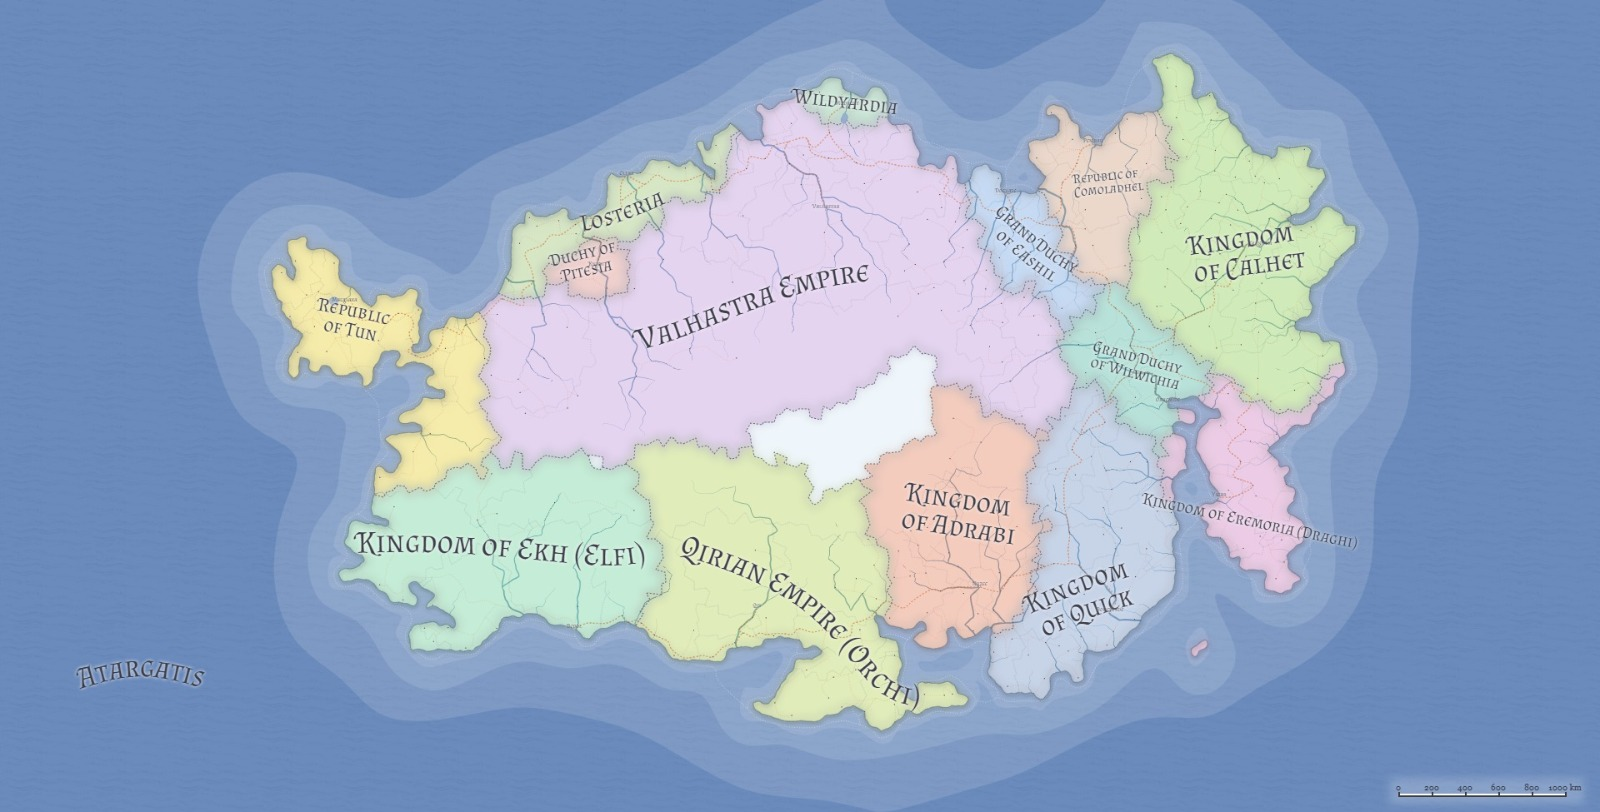
\includegraphics[scale=0.3]{mappaValhastra.jpeg}
\newpage

All' interno del singolo continente pangea abbiamo:

\begin{itemize}

\item{Impero di Valhastra}
\item{Impero Quirian}
\item{Regno di Ekh}
\item{Regno degli Adrabi}
\item{Regno del Quick}
\item{Granducato di Eashil}
\item{Granducato di Wilwichia}
\item{Regno di Calhet}
\item{Repubblica di Comholadel}
\item{Regno di Eremoria}
\item{Wildyarda}
\item{Losteria}
\item{Ducato di Pitesia}
\item{Repubblica del Tun}
\item{Atargatis}
\item{Zone bianche proprietà di nessuno}

\end{itemize}

\subsubsection{L'impero di Valhastra}

L'impero di Valhastra controlla la più vasta area mondiale, rappresenta una delle superpotenze del mondo assieme all' impero Quirian,il regno di Ekh,il regno degli Adrabi e il regno del Quick, in quest'ordine di potenza.
Nell' impero risiedono creature umanoidi bipedi miste come umani, elfi, orchi, mezzelfi, mezzorchi e altre creature minori, in totale armonia senza differenze.
Ognuna di esse si porta con sè secoli di cultura,religione e storia, ma rimangono fuse in un melting pot poichè le grandi città dell'impero riescono a custodire strutture adatte a bisogni comuni e singoli delle varie etnie.
La città più importante ospitata dall'impero è l'omonima città di Vahlastra, la capitale che ospita anche il castello della famiglia imperiale, composta dall'imperatore Tolomeo Valhastriss, rimasto vedovo senza regina, ma con cinque figlie dalle abilità artistiche e combattive eccellenti, il fiore all'occhiello dell'impero.

Di seguito viene presentato un modello che raffigura la capitale di Valhastra, fulcro importante di partenza per decine di avventure:

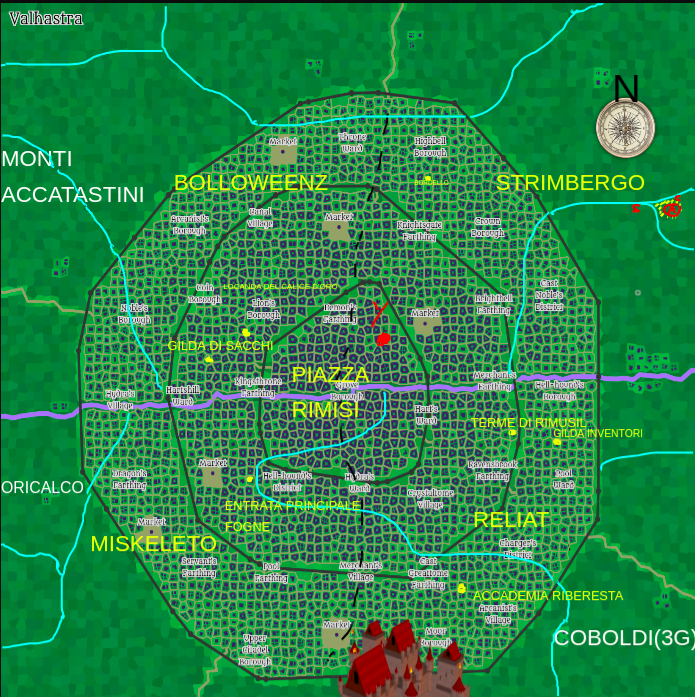
\includegraphics[scale=0.9]{PiantinaValhastra.png}
\newpage

è possibile notare come la città sia divisa principalmente in quattro distretti: Bolloweenz,Strimbergo,Miskeleto,Reliat, rispettivamente il distretto residenziale e delle gilde, il distretto più malfamato, il distretto dove vi sono perlopiù strutture religiose e il distretto elittario dove abitano i nobili e dove più a sud risiede il castello imperiale, posto su un rialzamento montuoso.
Nel centro della città sorge anche la piazza Rimisi, il luogo comune di tutti coloro che desiderano commerciare qualsiasi tipo di bene, in genere i negozi si concentrano in quell'area, dalle bancarelle di esposizione a veri e proprio edifici acquistati o affittati a qualche nobile.
In bianco sono segnate alcune possibili destinazioni che i giocatori hanno già raggiunto durante le loro precedenti avventure, la mappa infatti è in continuo cambiamento.

\subsubsection{L'impero Quirian}

L'impero Quirian è definito così perlopià per la potenza di attacco di cui è dotato, infatti si hanno poche informazioni sul modello politico che esso veramente detiene.
Esso è governato e popolato principalmente da Orchi, vissuti secoli prima in totale isolazionismo e pace con le altre nazioni, però poi per qualche fatto non noto ancora alla popolazione comune è scoppiata una furiosa guerra tra esso da un lato e l' alleanza tra l'impero di Valhastra e quello degli elfi dall'altra.
Questa guerra continua da decenni,dove le popolazioni hanno tentato di rubarsi i territori ma senza troppi risultati, infatti le zone bianche presenti sulla mappa politica mondiale rappresentano zone vuote devastate dai conflitti, ormai impraticabili per qualsiasi tipo di costruzione o forma di agricoltura.
Negli anni l'impero di Valhastra ha continuato a resistere con lo scopo un giorno di penetrare nelle difese dell'impero orchesco per fermare l'avanzata nemica ma con scarsi risultati.
Il morale degli uomini al fronte infatti è diventato sempre più cupo e svolgiato.
Quello che si sa è che è una popolazione molto tribale ma se non provocata non violenta fra i propri simili e non sciocca come altri fantasy possono stereotipare. Si dice infatti che esista una città nei meandri dell'impero che faccia da capitale e abbia diversi punti a favore a livello tecnologico rispetto a quelli di altri stati.
A livello politico, il regno del Adrabi inizialmente dette il suo contributo all'impero nella guerra, ma non vedendo un bagliore di soluzione decise col tempo di realizzare un muro impenetrabile tra sè e gli orchi per impedire loro di avvicinarsi alle loro terre.

\subsubsection{Il regno di Ekh}

Esso consiste in un regno dove la maggior parte delle cose sono basate sulla magia.
I ricercatori più importanti sono quasi tutti elfi poichè la loro aspettativa di vita è diverse volte più ampia quella di un comune umano.
Gli elfi sono una popolazione molto orgogliosa e sono disposti a collaborare con chi detiene il potere con forza, come l'impero di Valhastra ma condannano pienamente coloro che vivono da selvaggi, vista da loro come quasi una malattia.
Le città elfiche sono molto particolari, intrinse di potere magico e dove abbonda sempre principalmente la cultura locale.
Sono anche un simbolo importante per il turismo poichè è la nazione con più costruzioni particolari, molte delle quali utilizzate per i rituali più disparati.

\subsubsection{Il regno degli Adrabi}

Gli Adrabi regnano in un clima che si fa sempre più desertico andando a est.
La loro fortuna è essere quasi gli unici a riuscire facilmente a stabilirsi in un luogo così aspro per tradizione orale e pratica.
La loro cultura non impone loro di riunirsi in città enormi ma piccoli villaggi oppure di essere nomadi in cerca di fortuna.

\subsubsection{Il regno del Quick}

In questo regno abitano tre categorie di creature: gli spiriti (pixie, fate, fantasmi..) ,gli animali intelligenti e i druidi, persone di qualsiasi etnia che hanno deciso di vivere a stretto contatto con la natura e di effettuare un eterno scambio magico con essa.
Il governo è degli spiriti ma è equalitario nei confronti degli altri due. Gli animali sono l'80\% della popolazione.

\subsubsection{Il granducato di Eashil}

Questo granducato viene definito tale poichè col tempo si è sempre più isolato ma non copre un'area vasta come quella di un regno, ne troppo angusta come quella di un ducato più semplice.
La sua storia è ricca di mistero, poichè diversi portali verso altri piani si sono aperti nel corso del tempo, deturpando l'equilibrio climatico,fisico,chimico e magico dell'area.
Infatti è possibile trovare una ricca presenza di laghi d'acido,fiammelle verdeacqua,erbe di colore azzurro,pietra di colore rossiccio che viene utilizzata per costruire mura ed edifici, cambi repentini e veloci di temperatura.
In questa zona regnano gli Xibiati , una famiglia che ha preso il potere e regna su queste creature comparse da chi sa dove.

\subsubsection{Il granducato di Wilwichia}

è un regno composto da violenti giganti, in continuo tentativo di ascesa contro gli altri stati, vogliono governare ma non hanno una struttura effettivamente consona per farlo. Sono perlopiù barbari ma la strategia tendenzialmente vince sui loro grandi corpi.

\subsubsection{Il regno di Calhet}

è un regno per soli umani, dove solo alcune eccezioni etniche sono possibili. Mirano alla conservazione del ``Sangue pure'' a loro dire, ma per il resto sono una buona potenza militare, con un paese che nel loro vincolo è libero e ben trattato.
La famiglia reale è numerosa.

\subsubsection{Repubblica di Comholadel}

è un regno che si divide in due zone principali, quella costiera e quella nell'entroterra.
è un regno abitato da etnie miste unite da un'unica storia, quella del capitano pirata  Trutter, anticamente custode di un grandissimo tesoro, che si diresse sulle coste dell'attuale repubblica e decise di stabilirsi lì per amore, utilizzando i suoi averi per costruire il suo regno.
Col passare degli anni lui si ammalò e morì apprezzato dalle popolazioni locali che decisero di istituire un governo repubblicano in suo onore.
Attualmente è un governo in pace se non per qualche battibecco con il granducato di Eashil.

\subsubsection{Il regno di Eremoria}

è un regno dove prevalentemente abitano i draghi, esseri dall'intelletto sopraffino,dalle abilità magiche sorprendenti e da altrettanto orgoglio.
Governano le terre con una gerarchia di capo alpha, ma entrano in conflitto con altri solamente in caso il proprio avversario gli interessi.

\subsubsection{Wildyarda}

è un regno al momento quasi anarchico, composto da coloro che sono stati scacciati dal regno di Calhet e che per mare sono arrivati sulle coste a nord dell'impero di Valhastra.
Fondamentalmente sono associati all'impero stesso, che li supporta leggermente per le questioni finanziarie.
Tendenzialmente sono un popolo povero, di poco interesse per le altre nazioni.

\subsubsection{Losteria}
Losteria è un paese governato da un'oligarchia ricca, che si è impadronita nei secoli dell' egemonia marittima e primeggia nel settore della pesca e del trasporto via nave di merci verso altri paesi.
Qui di di denaro ce n'è molto e di conseguenza il costo della vita è parecchio caro, ha un ottimo rapporto con l'impero di Valhastra e questo è per entrambi un enorme vantaggio per collegare commercio marittimo e commercio su terreno all'interno del continente

\subsubsection{Il ducato di Pitesia}
é la seconda comunità di giganti all'interno dell'ambientazione. Le leggende narrano che la spaccatura fra le popolazioni del ducato di Pitesia e del granducato di Wilwichia sia avvenuta centinaia di anni prima la comparsa delle popolazioni ora conosciute e accadde a causa di un importante conflitto che ridusse di molto il valore demografico di entrambe le popolazioni, tuttavia ormai entrambe si suppone abbiano dimenticato questa storia riscrivendone una loro per ciascun ducato. Ha un rapporto neutrale con l'impero di Valhastra.

\subsubsection{La repubblica del Tun}

La repubblica del Tun è fondata sugli onori e le pratiche degli antichi samurai che, a confronto con la realtà, imitano ma mischiano la cultura giappo-cinesi creando una simile (La cosa in realtà non è ancora stata approfondita chiaramente poichè non è necessità primaria al momento ai fini della trama del gioco).
L'unica cosa che veramente potrebbe variare è il modello politico, molto più moderno dove il presidente del consiglio lascia spazio al maestro spadaccino e il consiglio è l'assemblea governativa ed è unica per tutti i poteri politici.

\subsubsection{Atargatis}

Atargatis è un regno formato da creature marine intelligenti, alcune tali da essere parzialmente umanoidi come ad esempio le sirene.
Questo luogo è oggetto di studio e aperta diplomazia poichè è stato rinvenuto nelle profondità marittime solamente negli ultimi anni.
Questo regno è molto vasto e strategicamente molto comodo per gli abitanti di Atargatis poichè posto sott'acqua, a diversi metri di profondità e in mezzo a tre correnti marine di differente direzione e verso, tutte molto forti, ad eccezione di un alcuni punti dove la situazione è più calma e vengono chiamati punti d'ingresso con l'omonima funzionalità pratica.

\subsection{La ruota dei piani}

La grande ruota è un modello convenzionale adottato dagli studiosi del piano materiale per indicare la posizione dei piani e per elencarli e distinguerli, tuttavia come già ribadito i piani sono realtà alternative che si distribuiscono come strati sottili di una torta o come una risma di fogli appoggiati uno sopra l'altro.
Possiamo definire come piani interni, le dimensioni alternative al piano materiale che si avvicinano perlopiù alla ``parete dimensionale'' o che nella cosmologia comune concepita dagli studiosi del piano materiale sta più vicino al centro (che coincide con il piano materiale stesso).
L' immagine seguente mostra anche la presenza anche dei piani esterni, ovvero quelli più lontani, che appaiono come più difficilmente raggiungibili e in alcuni casi estremamente differenti dal piano materiale.
Ogni ambientazione in sè può contenere i propri piani concepiti dall' autore dell'universo narrativo, tuttavia per semplicità si possono scegliere piani standard già appartenenti a famose ambientazioni fornite dagli stessi sviluppatori del gioco,come in questo caso.
Infatti in particolare, piano materiale a parte, viene adottata dall'ambientazione di Valhastra la cosmologia dell'ambientazione di Greyhawk.

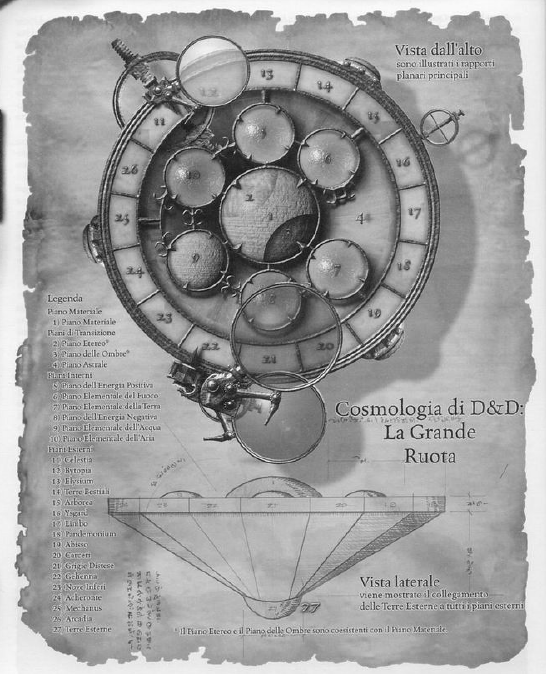
\includegraphics[scale=0.7]{Piani.png}
\newpage

Questa immagine appartiene ad una delle pagine del \textbf{Manuale dei piani 3.0}, ovvero il manuale della cosmologia standard di D\&D terza edizione, prima dell ` aggiornamento a quella 3.5.
Consiglio per descrizioni sicuramente più approfondite la lettura di quest'ultimo.
Per semplicità sono stati racchiusi tra i piani interni anche quelli di transizione nell' immagine per una questione di semplicità.

\subsection{I piani interni}

Vengono distinti ora i piani tra interni ed esterni, riprendendo i numeri dell'immagine qui sopra, seguono brevi descrizioni.
All' interno dei piani interni abbiamo:

\begin{enumerate}

\item{Il piano materiale}
\item{Il piano etereo}
\item{Il piano delle ombre}
\item{Il piano astrale}
\item{Il piano dell'energia positiva}
\item{Il piano elementale del fuoco}
\item{Il piano elementale della terra}
\item{Il piano dell' energia negativa}
\item{Il piano elementale dell'acqua}
\item{Il piano elementale dell'aria}

\end{enumerate}

\subsubsection{Il piano etereo}

Questo piano rappresenta un piano invisibile posto subito al di sopra del piano materiale.
è interessante poichè fornisce una visione leggermente distorta del piano materiale in sè e coloro che vi entrano invece appaiono invisibile dal piano materiale e anche non provocano rumore, come dietro ad un vetro insonorizzato per qualche motivo.
Oltre a ciò descritto questo piano ospita nebbie e nubi colorate.

\subsubsection{Il piano delle ombre}

Questo è un piano oscuro, tetro ma non per forza ricco di forze maligne. è ricco di confusione e può mutare in qualsiasi momento, esso contiene tutto ciò che è dimenticato e diroccato, tutte quelle creature il cui scopo è stato perduto e soprattutto una profonda oscurità. è facile perdersi nel piano delle ombre, tuttavia un buon studioso planare sa che è un piano estremamente utile per gli spostamenti fra realtà parallele del piano materiale e per affrontare lunghe distanze nella realtò di partenze(un passo nel piano delle ombre conta diversi passi compiuti nel piano materiale).

\subsubsection{Il piano astrale}

Il piano astrale è tutto ciò che si frappone tra un piano ed un altro, contiene molto vuoto, ma anche nuvole cilindriche, vortici di vento e fulmini in alcuni casi.
Qualsiasi incantesimo o sistema magico-tecnologico che consente una trasporto planare passa momentaneamente per il piano astrale.

\subsubsection{Il piano dell'energia positiva e il piano dell'energia negativa}

Questi due piani sono all' opposto. Infatti il piano dell'energia positiva concentra dentro di sè una grandissima quantità di magia, di luce, di energia, di vita, paragonabile a una stella, mentre viceversa il piano dell'energia negativa è un piano di tristezza e debolezza, dove la magia, l'energia e la vita scarseggiano, mantenendo un profondo equilibrio con il precedente.

\subsubsection{I Piani elementali}

I piani elementali del fuoco,dell'acqua,della terra e dell'aria rappresentano la casa dei mostri e delle creature fatte o orientate pesantemente a questi elementi.
Sono distese concentrate di questi quattro elementi che si estendono per kilometri e kilometri.

\subsection{I piani esterni}

I piani esterni sono quelli più particolareggiati e lontani dal piano materiale e sono:

\begin{enumerate}
\setcounter{enumi}{10}

\item{Celestia}
\item{Bytopia}
\item{Elysium}
\item{Terre bestiali}
\item{Arborea}
\item{Ysgard}
\item{Limbo}
\item{Pandemonium}
\item{Abisso}
\item{Carceri}
\item{Grigie distese}
\item{Gehenna}
\item{I nove inferi}
\item{Acheronte}
\item{Mechanus}
\item{Arcadia}

\end{enumerate}

\subsubsection{Celestia}

Celestia è un monte enorme fluttuante nei cieli più luminosi ed è equiparabile al paradiso nella concezione occidentale reale.
Esso è composto da sette cieli e accoglie livelli di luce sempre più abbondanti.
è terra di legge, di rispetto, di pietà ,di bonta, di pace suprema.

\subsubsection{Bytopia}

Bytopia è un piano formato da due forze di gravità contrastanti modellate su due strati di materia posti uno di fronte all'altro.
Queste forze di gravità non agiscono sugli stessi punti del piano, bensì sulla loro metà, tuttavia sono di uguale direzione ma di verso contrario come nell'immagine seguente.

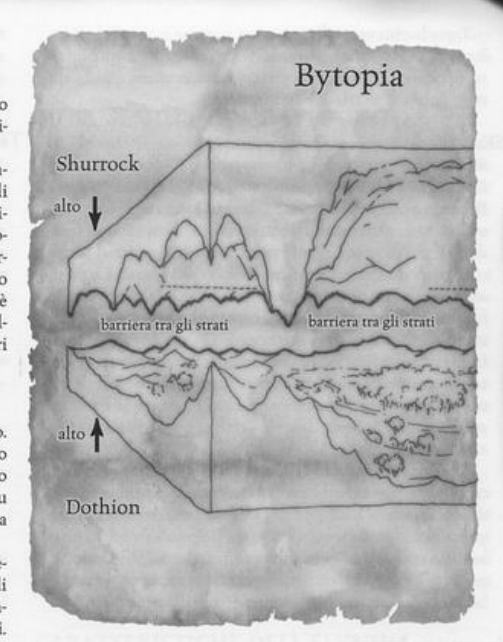
\includegraphics{Bytopia.png}
\newpage

Non appena una creatura attraversa l'invisibile linea di separazione fra i due strati, essa cade per la forza di gravità dell'altro strato.
è una terra abitata praticamente quasi tutta da gnomi.

\subsubsection{Elysium}

I campi benedetti dell'Elysium sono paragonabili all' Eden della religione cristiana con qualche modifica.
è un luogo bucolico, dove chi ci entra ne rimane affascinato sia per i luoghi, sia per la magia che mette l'altruismo sopra ogni pratica e in modo costante.
è un luogo dove chi ci entra non vuole più tornare a casa solitamente, un luogo dove la pace è assicurata.

\subsubsection{Le terre bestiali}

è il piano dove si dirigono le anime degli animali caduti.
è un regno di foreste altissime e fittissime, di deserti pieni di vita a differenza dell'esempio classico, di pini enormi innevati, di arbusti e cespugli disposti ovunque, un luogo dove tutti gli animali possono vivere in pace e la natura cresce rigogliosa e senza limiti.

\subsubsection{Arborea}
Molto simile alle terre bestiali, Arborea ha come differenze il fatto di ospitare anche enormi campi fioriti e invece degli animali ospita gli elfi dei boschi, ospitando soprattutto i signori degli elfi.

\subsubsection{Ysgard}
Ysgard è la terra degli eroi, simile a quella riportata dalla mitologia nordica vichinga.
è un luogo di climi difficili e battaglie eterne dove sono appunto gli eroi possono sopravvivere.
è formato da isole sospese e fiumi di terra grandi come continenti, laghi di fuoco e cadute di neve pesanti.

\subsubsection{Limbo}

è il tutto e il nulla, è caos puro.
All' interno del limbo si racchiudono frammenti di realtà provenienti da ogni angolo della ruota e dove gli elementi si fondono mutando e creare cose nuove che successivamente vengono rimodellate subendo nuovi stimoli all'infinito

\subsubsection{Pandemonium}

è un luogo senza luce fatto di caverne in cui scorre in modo continuativo un vento che, per la morfologia del luogo, produce urla e ululati continui e sovrapposti, portando chi ci entra alla follia.
Qui giacciono infatti creature ormai folli che cercano nuovi individui per sottoporli alla loro follia.
è un luogo di grida, dove non si riesce a parlare e a comunicare.
è un luogo freddo, dove ogni fuoco acceso viene spento dal vento.

\subsubsection{Abisso}

è il luogo dove la malvagità e l'orrore regnano sovrani.
è il luogo dove vi sono creature striscianti e creature malvagie come i demoni.
è il luogo dove l'etica viene abbandonata.
è un piano formato da centianaia di strati in cui si può cadere ripetutamente finendo in un baratro di orrore sempre peggiore.

\subsubsection{Carceri}

è un luogo malvagio, la prigione definitiva, il luogo dell'esilio, dimore della divinità della morte Nerull.

\subsubsection{Grigie distese dell'Ade}

è il luogo dove perdurano infinite battaglie sanguinose tra diavoli e demoni.
è un posto dove la sofferenze e la disperazione di chi ci entra sale alle stelle.

\subsubsection{Gehenna}

è un luogo ricco di lava, dove diverse isole dotate di vulcani sorvolano l'ammasso di magma sottostante.
In questo clima delle popolazioni sono riuscite nei secoli a creare delle città ma resta comunque al momento un luogo difficilmente vivibile.

\subsubsection{I nove inferi}

Sono molto simili ai nove inferi danteschi, vi è lo stige e i dannati sono ospitati e torturati dai diavoli che abitano quelle terre.

\subsubsection{Acheronte}

è uno dei luoghi di battaglia eterna, è dove finiscono le ribellioni maggiori, dove l'ordine militare è più importante di qualsiasi etica e dove lo scontro quindi, è inevitabile.

\subsubsection{Mechanus}

è un piano legato in modo stretto con la tecnologia, la pianificazione, la progettazione e la logica.
è un piano ricco di ingranaggi,meccanismi e fortezze di metallo. Il luogo dove abitano i più grandi ingegneri del multiverso.

\subsubsection{Arcadia}

è il mondo della perfezione ,sia di perfetta armonia, sia di perfetta forma geometrica, infatti non ci sono imprecisioni e non possono esserci, è il mondo in cui nemmeno le montagne si erodono col tempo.

\saltariga
\chapter{Religioni del mondo}
\section{Religioni del mondo}

La religione è un aspetto importantissimo in dungeons \& dragons poichè può essere strumento del master per tessere la storia in modo più misterioso o mitico, può essere un motivo per cui dare un obbiettivo e soprattutto per i giocatori che scelgono la classe standard di chierico o paladino è essenziale, poichè il tipo di religione rappresenta per queste categorie le capacità magiche che essi possiedono.

\subsection{Magia divina}

La magia divina è quella forma di magia che proviene da un luogo più alto e tendenzialmente irraggiungibile, ovvero dagli dei stessi.
Non è obbligatoria la presenza di diverse divinità, può esistere anche solamente una divinità, ma il politeismo concede ai giocatori varietà di divinità e cammini quindi tra cui scegliere.
Come per i piani, le divinità adottate per l'ambientazione di Valhastra sono state prese da quella di Greyhawk, visto anche che alcune di esse sono in chiaro collegamento coi piani sopra citati.
Di seguito vi è l'elenco delle divinità con il rispettivo dominio e reliquia sacra rispettivi, il primo riguarda l'argomento principali su cui è concentrata l'essenza della divinità (luce, vita, fortuna, morte, dolore...), mentre il secondo è un oggetto fondamentale per i credenti che utilizzano magia divina di quella divinità.

\subsection{Divinità}

\subsubsection{Boccob}

Boccob è il dio della magia e della ricerca, è probabile che tutti gli oggetti magici esistenti ci siano grazie alle sue ricerche iniziali.
I suoi domini sono conoscenza,inganno e magia.
Il suo simbolo sacro è una forma a pentagono cava con solo i bordi con dentro un occhio di metallo.

\subsubsection{Corellon Larethian}

Corellon è il dio degli elfi,protettore e conservatore della vita.
I suoi domini sono bene,caos,guerra e protezione.
Il suo simbolo sacro è una mezzaluna.

\subsubsection{Ehlonna}

Elhonna è la dea delle terre boschive.
I suoi domini sono animale,bene,solo e vegetale.
Il suo simbolo sacro è la statuetta di un unicorno.

\subsubsection{Erythnul}

Erythnul è il dio del panico e del massacro.
I suoi domini sono caos,guerra,inganno e male.
Il suo simbolo sacro è una moneta con disegnata una caricatura di un umanoide con la testa abominevole.

\subsubsection{Fharlanghn}

Fharlanghn è il dio del viaggio.
I suoi domini sono protezione e viaggio.
Il suo simbolo sacro è un pezzo di corteccia con un disegno

\subsubsection{Garl Glittergold}

Garl Glittergold è il dio degli gnomi, conosciuto come il burlone, veglia sull' umorismo.
I suoi domini sono bene, inganno e protezione.
Il suo simbolo sacro è una pepita d'oro.

\subsubsection{Gruumsh}

Gruumsh è il dio degli orchi, malvagio,chiamato colui che non dorme mai, sostiene i forti e fa tremare i deboli, spinge a fare razzie e conquiste territoriali alle popolazioni
I suoi domini sono caos,forza,guerra e male.
Il suo simbolo sacro è una gemma a forma di occhio di colore violaceo.

\subsubsection{Heironeus}

Heironeus è il dio della giustizia.
I suoi domini sono bene, guerra e legge.
Il suo simbolo sacro è una mano che impugna una saetta.

\subsubsection{Hextor}

Hextor è il dio della tirannia, detto anche della distruzione.
I suoi domini sono distruzione, guerra, legge e male.
Il suo simbolo sacro è una mano che impugna delle frecce.
è il fratellastro di Heironeus.

\subsubsection{Kord}

Kord è il dio della forza, detto il lottatore, protegge gli atleti.
I suoi domini sono bene, caos, fortuna e forza.
Il suo simbolo sacro è un scudo dipinto.

\subsubsection{Moradin}

Moradin è il dio dei nani, spirito forgiatore, protegge le arti e le scienze della lavorazione del ferro e delle gemme preziose.
I suoi domini sono bene, legge, protezione e terra.ù
Il suo simbolo sacro è un'incudine con il martello.

\subsubsection{Nerull}

Nerull è il dio della morte, detto il mietitore.
I suoi domini sono inganno, male e morte.
Il suo simbolo sacro è un teschio.

\subsubsection{Obad-Hai}

Obad-Hai è il dio della natura, amico di tutti coloro che vivono in armonia con la natura.
I suoi domini sono acqua, animale, aria, fuoco, terra e vegetale.
Il suo simbolo sacro è un arbusto che assume la forma di un volto.

\subsubsection{Olidammara}

Olidammara è il dio dei ladri, detto il ladro ridente.
I suoi domini sono caos, fortuna e inganno.
Il suo simbolo sacro è una maschera mezza nera e mezza bianca con sopra disegnato un ghigno.

\subsubsection{Pelor}

Pelor è il dio del sole e della luce.
I suoi domini sono bene, forza, guarigione e sole.
Il suo simbolo sacro è un sole che assume la forma di una faccia umanoide.

\subsubsection{St. Cuthbert}

St. Cuthbert è il dio della legge e del castigo.
I suoi domini sono distruzione, forza, legge e protezione.
Il suo simbolo sacro è un medaglione circolare con inscritta una croce di metallo.

\subsubsection{Vecna}

Vecna è il dio dei segreti nascosti e come Boccob della conoscenza ma più occulta.
I suoi domini sono conoscenza, magia e male.
Il suo simbolo sacro è un occhio vero.
Di lui si sa che in qualche modo sia asceso come divinità attraverso la ricerca dell'occulto.

\subsubsection{Wee Jas}

Wee Jas è la dea della morte e della magia, chiamata la dea stregona.
I suoi domini sono legge, magia e morte.
Il suo simbolo sacro è una moneta con incisa sopra un volto demoniaco.

\subsubsection{Yondalla}

Yondalla è la dea degli halfling (gli hobbit per chi conosce il signore degli anelli), detta la benedetta.
I suoi domini sono bene,legge e protezione.
Il suo simbolo sacro è uno scudo che raffigura un cesto di frutta.

\subsection{Nota}

Tutte le divinità si possono trovare in modo più dettagliato a pagina 107 del \textbf{Manuale del giocatore di 3.5}.

\saltariga
\chapter{Altre forme di magia}
\section{Altre forme di magia}

Nonostante la magia divina sia stata la tipologia di magia prima presentata, nell'ambientazione di Valhastra sono presenti le forme standard di magia arcana e druidica.

\subsection{La magia arcana}

La magia arcana deriva da meccanismi interiori del proprio corpo che consentono lo scambio di energia con l'esterno. Questa energia via allenata per aumentarne la riserva  e può essere manipolata in modi molto diversi.
Grazie a questo principio di funzione è possibile lanciare incantesimi arcani oltre a quelli divini.

\subsection{La magia druidica}

Una branca della magia divina è quella druidica, che invece di arrivare da una divinità essa è presente in tutte le forme della natura, da animali a vegetali e viene utilizzata grazie a queste ultime componenti.

\saltariga
\chapter{Organizzazioni e istituzioni}
\section{Organizzazioni e istituzioni}

Nel mondo di Valhastra vi sono differenti organizzazioni e istituzioni differenti, tuttavia è importante considerare soprattutto quelle di Valhastra, da cui provengono i nostri giocatori.

\subsection{Un sistema a gilde}

All' interno delle città e di qualche villaggio maggiore vi sono le cosiddette gilde: ambienti dove studiosi, ingegneri, storici, mercanti, artigiani, manovali e avventurieri si iscrivevano per rispondere agli appelli della popolazione mediante contratto stipulato col capo gilda. La gilda esegue il servizio di trovare i compiti da svolgere e si trattiene parte del guadagno da essi.
La gilda ha anche il compito di formare i propri dipendenti.

\subsection{La guardia cittadina}

La guardia cittadina, a differenza di oggi, non è legata a Valhastra con l'esercito bensì come organizzazione a sè.
è composta da membri sia dell'esercito che da volontari qualsiasi che hanno passato gli esami necessari ad essere qualificati per aiutare la comunità. Non rappresenta un organo molto forte poichè le gilde col tempo affermandosi sempre di più hanno risolto i vari problemi per cui spesso le guardie non sono chiamate alle armi.
Nel caso di un attacco alla città , è priorità della guardia cittadina salvare la popolazione piuttosto che combattere, compito che spetta se c'è all'esercito. Nel caso di mancanza dell' esercito, la guardia cittadina si organizza anche per la difesa del luogo, coordinandosi con le gilde di avventurieri.

\subsection{L` esercito}

L' esercito è formato come nella realtà da sezioni interne di gruppi di soldati.
I soldati si differenziano anche per il ruolo che coprono al suo interno.

\subsubsection{La fanteria}

La fanteria si compone di unità tutte di terra tendenzialmente non con elevate capacità magiche e si suddivide in coloro che utilizzano armi ravvicinate o armi a distanza.

\subsubsection{La cavalleria}

La cavalleria si occupa di effettuare spostamenti di velocità superiore alla fanteria, sono i primi a entrare in battaglia nei punti importanti, essi posso determinare molto la strategia adottata da un esercito.

\subsubsection{I maghi da  combattimento}

L' unità dei maghi da combattimento è molto ristretta e a differenza delle altre unità che formano truppe da centinaia se non migliaia di soldati al colpo, i maghi da combattimento sono circa una ventina per ogni squadra e hanno la possibilità di scagliare importanti magie sul nemico, alcune con pesanti risultati. Hanno anche il vantaggio di poter incanalare il loro potere magico dentro delle sacche zaino che permettono loro di volare per un' ora e intervenire dall'alto su alcune aree ben precise.
Rappresentano un po' la soluzione area moderna.

\subsubsection{I difensori}

I difensori sono un' unità utilizzata perlopiù nella guerra tra l'impero di Valhastra e quello degli orchi.
Il loro scopo è quello di avanzare lungo il confine di battaglia trasportando grandi scudi molto pesanti.
Purtroppo la pesantezza degli scudi permette loro spostamenti in lunghi tempi, ma sono necessari poichè, spostandosi in linea retta o comunque un perimetro, essi letteralmente spostano il confine dell'impero verso sud.
Nel momento in cui tutti gli scudi vengono piazzati a terra, viene definita magicamente una nuova barriera magica , spostata rispetto alla precedente, ricavata dalla riserva magica contenuta all'interno degli scudi e rilasciata solo alla fine dello spostamento.

\subsubsection{I navigatori}

I navigatori sono un' unità di studiosi che si occupano di intercettare eventuali invasioni del nemico da un piano differente a quello materiale, per evitare assalti a tenaglia da vari punti.
Loro con un sistema di intercettazione convergono il teletrasporto dei nemici in punti specifici dove possono eliminarli in modo veloce e sicuro.

\subsubsection{Unità di spionaggio}

L'unità di spionaggio si occupa di invadere altri stati con lo scopo di raccogliere informazioni importanti.

\subsection{La guardia imperiale}

La guardia imperiale è formata da combattenti formidabili, il cui equipaggiamento è stato forgiato con la massima cura e funzionalità.

\subsection{Le streghe del potere}

All' interno del mondo di Valhastra vi furono otto streghe che vagarono mille anni prima degli eventi contemporanei per il mondo ottenendo diverso potere dalle abitudini nefaste degli esseri senzienti.
Queste streghe si fecedero denominare le streghe dei peccati capitali e arrivarono quasi a diventare potenti come gli dei.
Gli dei tuttavia, più saggi e longevi le fermarono con una lotta che portò il mondo all' era in cui ci si trova adesso.
Il loro destion fu un mistero, ad eccezione della strega dell' avidità , Avezia, di cui la morte fu data per certa, tuttavia ella creò con il suo potere una versione magica di se stessa che la tenesse in vita solo in modo spirituale, conservando il suo spirito in un tempio di un villaggio fra le montagne, poco distante dalla capitale imperiale. 

\subsection{L` organizzazione oscura}

L' organizzazione oscura è stata fondata in circostanze sconosciute solo di recente e conta fra le proprie fila diverse tipologie di creature e persone dalle intenzioni maligne.
Il loro scopo è quello di abbattere il centrismo del piano materiale, spartendosi le terre tra i vari piani rimasti.
Gli ideali che vi sono fra i membri, non rispecchiano tutte le popolazioni extra planari, ma comunque una buona parte e sono bollati sul piano materiale da tutti gli stati come terroristi.
Si sa che un uomo mezzo elementale del fuoco comandi i loro affiliati, ma per il resto si sa gran poco di essi.

\saltariga
\chapter{Il tempo}
\section{Il tempo}

\subsection{La linfa dell' albero sacro}

Il tempo scorre all'interno di tutta Valhastra in modo quasi uniforme in tutti i piani.
Si può considerare il flusso degli eventi come la linfa di un albero sacro che scorre in vari punti, nel centro dell'albero, in tutto il tronco, nei rami e nelle foglie. Questa suddivisione non è casuale, infatti
in ogni punto dell'albero è presente una possibile realtà parallela, differente per anche una singola caratteristica rispetto alle altre.
Con realtà parallela si intende un luogo dove gli eventi si sono verificati in modo leggermente diverso da una realtà qualsiasi di partenza diversa da essa, il cambiamento può essere importante coem un catalisma o una riforma di stato, oppure meno impattante come una porta aperta che mi prima era chiusa.

\subsubsection{Le foglie}

L' albero in sè è parecchio imponente, in altezza e in età potrebbe essere considerato infinito addirittura, poco sanno infatti gli studiosi.
Nelle foglie di uno stesso ramo vi sono custodite realtà che cambiano molto poco fra di loro, con un impatto quindi contenuto.

\subsubsection{I rami}

I rami contengono invece realtà molto diverse fra di loro, pure in cui il continente di Valhastra venga mutato in modo diverso, rendendo quasi inutile questo documento

\subsubsection{Il tronco}

Si vocifera che nel punto più centrale del tronco, a fare da perno per le altre realtà vi sia la verità, la realtà da cui è cominciata la grande ramificazione.
Si dice che i nuovi boccioli dell'albero caddero nelle realtà formate dai rami come stelle che si spezzarono generando vita e futuro.
Si dice anche che esistano degli esseri in grado di viaggiare nel tempo attraverso tre tipologie di stratagemmi e che questi esseri siano provenienti dalla realtà madre. Essi vengono definiti invarianti, poichè appartengono ad una singola realtà senza esistere nelle altre e vengono da quella di partenza.

\subsection{Il viaggio nel tempo}

Ci sono tre tipologie di viaggio nel tempo che gli studiosi hanno teorizzato ma mai applicato:

\begin{itemize}

\item{Il loop --> un viaggio nel flusso della stessa foglia, ripete da capo una giornata ma non ci sono spostamenti di realtà}
\item{Lo spostamento temporale moderato --> spostamento da un ramo ad un altro oppure da una foglia ad un'altra foglia, il cambiamento è basato sulla differenza tra le realtà}
\item{Lo spostamento temporale pesante --> spostamento da un ramo ad un altro molto lontano oppure accesso al tronco ,oppure spostamento pesante di diversi anni nella foglia, solo nell'ultimo caso non c'è un cambiamento di realtà}

\end{itemize}

\section{L' artefice di Eberron}

\subsection{Guida all' utilizzo}

In questa ambientazione si fa uso di alcuni elementi di tecnologia steampunk (treni a vapore, armi da fuoco grezze, particolari meccanismi realizzati con le meccaniche degli orologi e degli ingranaggi) e l' artefice è la figura di spicco per l' utilizzo di questa componente abbinata alla magia.
Assieme alle classi base del manuale del giocatore di 3.5 e altre scelte da parte del giocatore parlandone col master su cui non voglio troppo soffermarmi, l' artefice rappresenta un personaggio anche complesso da giocare, soprattutto per un giocatore novellino, per cui ho deciso di integrare una parte relativa al funzionamento di questa classe.
Le prossime informazioni sono state prese dal \textbf{Manuale dell' ambientazione di Eberron per 3.5}.
L' artefice non è una classe magica (lo stregone ad esempio lancia incantesimi per cui lo è), ma è una classe che emula ed inganna il sistema magico attraverso la combinazione di tecnologia e magia.
Fra le capacità importanti acquisite dall' artefice la parte complessa riguarda la creazione degli oggetti magici.
Consiglio di consultare la sezione degli oggetti magici del \textbf{Manuale del dungeon master di 3.5}.
Dato un oggetto dalla tabella degli oggetti magici in vendita l'artefice deve spendere denaro,punti riserva dell' artefice e tempo per provare a fare l' oggetto in sè, con la possibilità anche di non riuscirci e dover riprovare.
La riserva dell' artefice è un contenitore di tot punti segnalato dalla sezione apposita dell' artefice nella tabella di avanzamento del livello sul manuale dell'ambientazione di Eberron.
Le formule da utilizzare sono le seguenti:

\begin{itemize}

\item{ $denaro = denaro - prezzoBase / 2$ per ogni tentativo}
\item{ $puntiRiserva = puntiRiserva - prezzoBase / 25$ per ogni tentativo}
\item{ $totGiorni =  max( prezzoBase/1000 , 1)$ per ogni tentativo}

\end{itemize}

Una volta applicati questi calcoli l'artefice tira un D20 e somma il suo valore di  utilizzare oggetti magici per riuscire a realizzare l'oggetto.
Se realizzato è pronto all'uso da qualsiasi personaggio che si intenda un minimo di magia.

\subsection{Esempio}

\begin{tabular}{|l|l|l|}
\hline
Artefice& Riserva&Denaro\\
\hline
Liv2 & 40&30.000\\
\hline
\end{tabular}

\saltariga
\saltariga

\begin{tabular}{|l|l|}
\hline
Oggetto& PrezzoBase\\
\hline
Bacchetta di palla di fuoco 50 cariche & 11.250\\
\hline
\end{tabular}

\saltariga
Otteniamo:

\begin{itemize}

\item{ $ denaro = denaro - (11.250 / 2)  = 30.000 - 5.625 = 24.375 $}
\item{ $ riserva = riserva - (11.250 /25) = 40 - 450 = - 410 $}
\item{ $ totGiorni = round(11.250 / 1000) = 11 $ }

\end{itemize}

Notare come la riserva sia andata in negativo!!!
\saltariga

In questo caso l'artefice può sottrarre i 410 punti rimasti dai suoi punti esperienza. Essendo al livello 2 significa che ne possiede almeno 1000 per cui rimarrà con un minimo di 590 punti esperienza, inoltre questo è solo per un tentativo, il calcolo va ripetuto per ogni tentativo dichiarato dal giocatore.
L'artefice poi può rivendere l'oggetto al prezzo che vuole realizzando così una possibile attività commerciale molto fruttuosa.

\end{document}